% Numerical results of the factorized Pauli--Villars multigrid (input by MDWF_MULTIGRID_NOTE.tex
% with \resultstrue). Every number is from a log named in the text; [TODO] marks what is still
% being measured.
\newcommand{\todo}[1]{\textcolor{red}{[TODO: #1]}}

% ============================================================
\section{Numerical results}
\label{sec:results}

\subsection{Setups}
\label{sec:setups}

\begin{table}[t]
\centering
\caption{The two setups and the multigrid of the mass scan. All runs: M\"obius
$(b,c)=(1.5,0.5)$, $L_s=8$, $m_{\rm PV}=1$, $\alpha_{\rm PV}=1$, boundary
$(1,1,1,-1)$, $\alpha=0.6$ unless stated. Configurations: quenched, plaquette action at
$\beta=6.0$, on $12^4$, $16^4$, $24^4$ and $24^3\times48$, four each; their plaquettes, $t_0$ and
topological charges are in Appendix~\ref{sec:configs}.}
\label{tab:setups}
\renewcommand{\arraystretch}{1.15}
\begin{tabular}{@{}lll@{}}
\toprule
 & setup S (stout) & setup B (bare) \\
\midrule
$M_5$ & $1.0$ & $1.8$ \\
gauge smearing & stout, $\rho=0.1$, 3 steps & none \\
Chebyshev smoother $\nu$, $\kappa_s$ & $8$, $10$ & $12$, $30$ \\
\midrule
\multicolumn{3}{@{}l}{multigrid (both setups)}\\
aggregates & \multicolumn{2}{l}{$4^4$ ($24^3\times48$: levels below with super-blocks $2$, $3$)} \\
test vectors & \multicolumn{2}{l}{$32$ ($16$ filtered low modes of $\AR\dg\AR$, lifted to $\{s,\hat t\}$)} \\
setup & \multicolumn{2}{l}{filter 2 rounds; bootstrap 2 rounds of 4 FGMRES steps} \\
coarse solves & \multicolumn{2}{l}{single precision, $|r|^2/|b|^2<10^{-2}$; Pauli--Villars $\tau=10^{-3}$} \\
precision & \multicolumn{2}{l}{$\Pro$ half, cycle single, outer solver double} \\
outer solver & \multicolumn{2}{l}{GCR(2) on $\AL$ to $|r|^2/|b|^2<10^{-18}$} \\
\bottomrule
\end{tabular}
\end{table}

\paragraph{Numerical setup.} The quenched configurations use the plaquette action at $\beta=6.0$,
a lattice spacing of about $0.1$~fm (Table~\ref{tab:configs}). Results are means, medians or
ranges over the four configurations of each volume as the captions state; the solvers without the
multigrid and the pseudospectra use configuration~1. The two setups of the M\"obius operator
(Table~\ref{tab:setups}) share $(b,c)=(1.5,0.5)$, the choice of the JLQCD and the RBC/UKQCD
Collaborations, and $L_s=8$.
\begin{itemize}
\item \emph{Setup B (bare links)} uses $M_5=1.8$, the value typical of simulations on unsmeared
links~\cite{Arthur2013}.
\item \emph{Setup S (stout links)} smears the links of the fermion operator (stout, $\rho=0.1$, three
steps, Sec.~\ref{sec:smearing}) and uses $M_5=1.0$, as in the JLQCD ensembles of
Ref.~\cite{JLQCDBpi}.
\end{itemize}
Both keep the near-zero modes of $W=D_W(-M_5)$ small, by moving $M_5$ (B) or by smoothing the
field (S), and so give the multigrid low modes of different character; they need different
smoother intervals (Table~\ref{tab:setups}). Timings are from one NVIDIA data-center GPU with
$24$\,GB of device memory; a second GPU was used for iteration counts and spectral quantities only.
The device reductions add in an order that depends on the build and the
GPU, so the iterations of otherwise equal runs can differ by a few. The setup seed is $21$ except
in Sec.~\ref{sec:pvcoarse}.

\subsection{Performance}
\label{sec:performance}

\subsubsection{Comparison with CGNE}
\label{sec:massscan}

On $24^3\times48$ the multigrid is $3.2$--$5.7$ times faster than mixed-precision CGNE at
$m=0.001$, and its setup is recovered within one point-source propagator for $m\le0.005$. We
compare first for one random right-hand side over seven masses, then for whole point-source
propagators.

\begin{figure}[t]
\centering
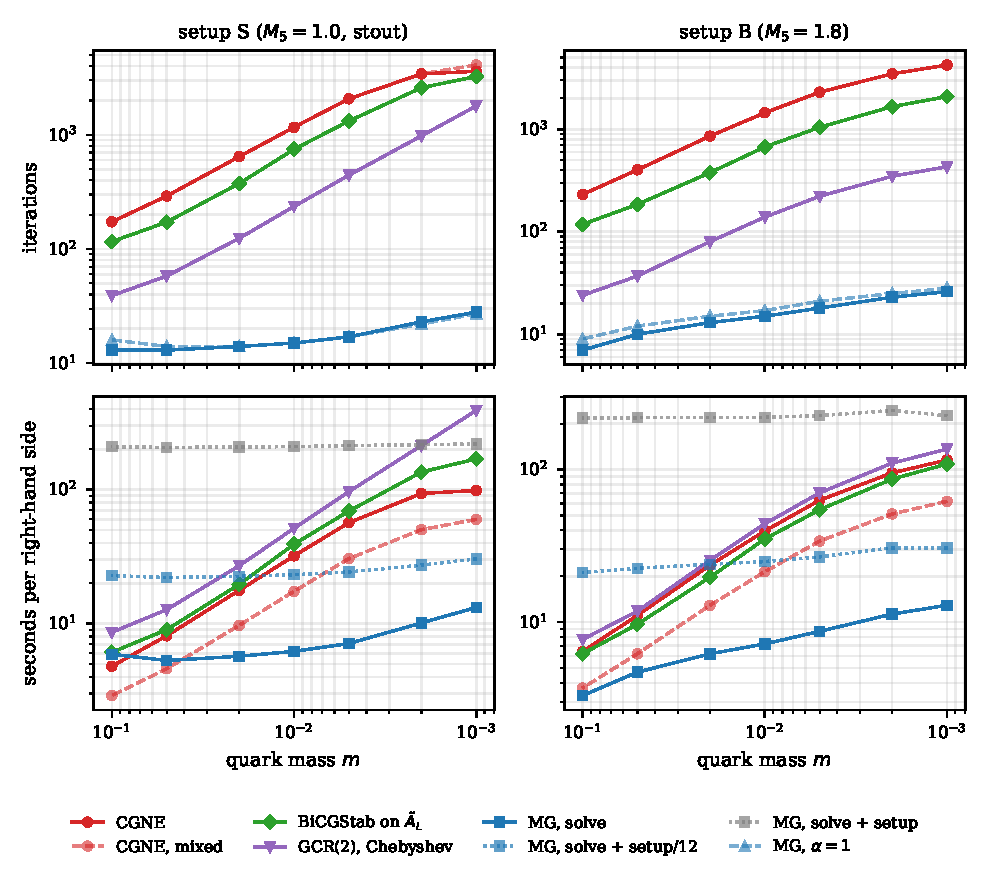
\includegraphics[width=\linewidth]{fig_massscan}
\caption{The mass scan of Table~\ref{tab:massscan}, the mixed-precision CGNE, and the Krylov
solvers on $\AL$ without the multigrid (Sec.~\ref{sec:nomg}): iterations (top) and seconds
per right-hand side (bottom) against the quark mass, $24^3\times48$. CGNE and multigrid: means over
the four configurations, bars from the smallest to the largest value; the solvers without the
multigrid: configuration~1. ``Solve + setup/12'': the setup spread over the 12 columns of one
point-source propagator.}
\label{fig:massscan}
\end{figure}

\paragraph{The reference solver.} It is CG on $\mathcal K\dg\mathcal K$, $\mathcal K=\Ce^{-1}S$,
the even-odd operator of Bridge++, with Neff's $\alpha$ as for the multigrid, in mixed precision.
Boyle and Yamaguchi~\cite{BY} used CG on $S\dg S$, which here needs more iterations
(Appendix~\ref{sec:cgform}).

\paragraph{Mass dependence.} The multigrid removes most of the critical slowing down of CGNE
(Fig.~\ref{fig:massscan}, Table~\ref{tab:massscan}). From $m=0.1$ to $m=0.001$ the iterations of
CGNE grow about twentyfold, those of the multigrid by $2.8$--$5.4$. Its setup is paid back after
$3.5$--$5.3$ right-hand sides at $m=0.001$. For $m\ge0.05$ in setup~S, CGNE is
faster or level. The multigrid needs three times the device memory of CGNE.

\paragraph{A point-source propagator.} At $m=0.001$ the multigrid takes $0.40$--$0.56$ of the wall
time of CGNE for a whole propagator, setup included (Table~\ref{tab:pointsource}). At $m=0.01$ the
setup is not quite paid back within the 12 columns. The pseudoscalar correlators of the two solvers
agree to $1\times10^{-6}$ or better.

\begin{table}[t]
\centering
\caption{Point-source propagators (12 columns) on $24^3\times48$: the multigrid
(setup seconds, iterations and seconds per column) against the mixed-precision CGNE
(iterations and seconds per column), the wall time of the whole propagator, and the
largest relative difference of the pseudoscalar correlator at $t=0\ldots3$. At $m=0.001$: ranges
over the four configurations and the 12 columns; at $m=0.01$: configuration~1.}
\label{tab:pointsource}
\renewcommand{\arraystretch}{1.12}
\setlength{\tabcolsep}{4pt}
\begin{tabular}{@{}lc ccc cc cc c@{}}
\toprule
 & & \multicolumn{3}{c}{MG} & \multicolumn{2}{c}{CGNE, mixed} & \multicolumn{2}{c}{wall (s)} & \\
\cmidrule(lr){3-5}\cmidrule(lr){6-7}\cmidrule(lr){8-9}
 & $m$ & setup & it & s & it & s & MG & CGNE & $|\Delta C|/C$\\
\midrule
S & $0.001$ & $203$--$222$ & $22$--$48$ & $11.1$--$26.4$ & $3634$--$6400$ & $52.1$--$91.6$ & $382$--$505$ & $678$--$1048$ & $\le1\times10^{-6}$\\
B & $0.001$ & $204$--$207$ & $22$--$30$ & $10.7$--$14.5$ & $4354$--$5574$ & $62.4$--$79.8$ & $363$--$398$ & $803$--$973$ & $\le7\times10^{-7}$\\
S & $0.01$ & $203$ & $16$--$17$ & $6.4$--$7.0$ & $1337$--$1388$ & $19.8$--$20.5$ & $305$ & $264$ & $2\times10^{-7}$\\
B & $0.01$ & $215$ & $17$ & $8.1$ & $1641$--$1745$ & $24.2$--$25.7$ & $331$ & $324$ & $4\times10^{-8}$\\
\bottomrule
\end{tabular}
\end{table}

\paragraph{Volume.} The advantage of the multigrid grows with the volume (Fig.~\ref{fig:volume},
Table~\ref{tab:volume}). It is slower than CGNE on $12^4$, about level on $16^4$, and clearly faster
from $24^4$ on: its iterations hardly grow with the volume, those of CGNE do. Its setup grows with
the volume.

\begin{figure}[t]
\centering
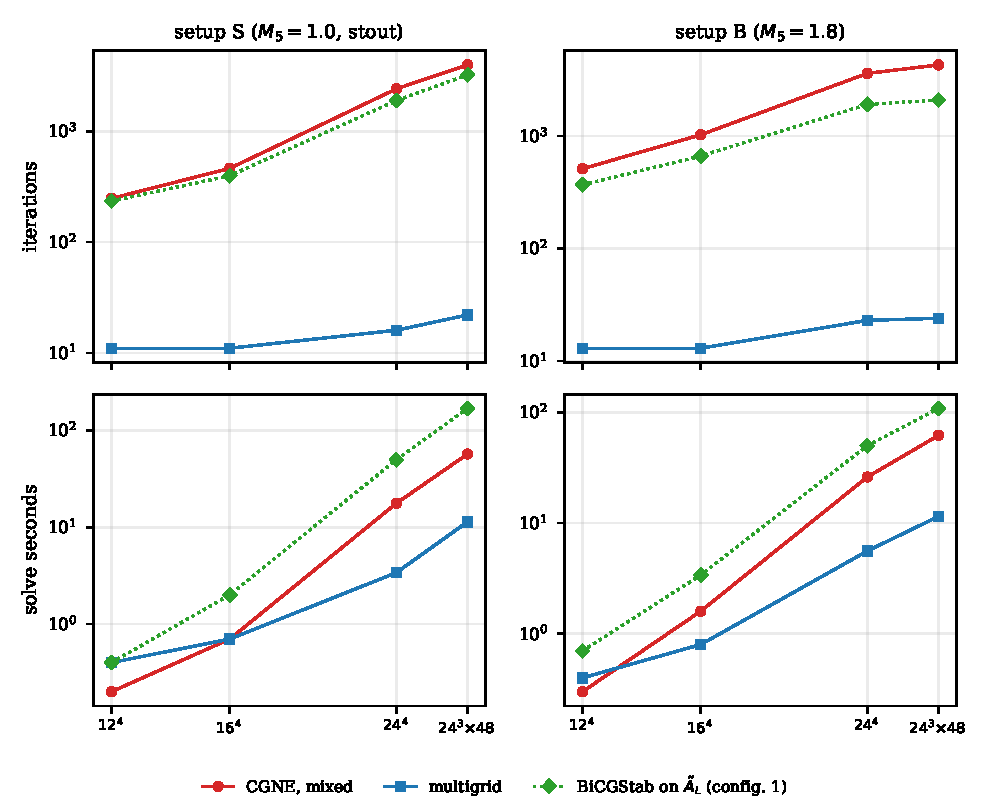
\includegraphics[width=\linewidth]{fig_volume}
\caption{Iterations (top) and solve seconds (bottom) at $m=0.001$ against the volume, one random
right-hand side. Mixed-precision CGNE and multigrid: median over the four configurations; BiCGStab
on $\AL$: configuration~1. The ranges are in Table~\ref{tab:volume}.}
\label{fig:volume}
\end{figure}



\paragraph{Neff's $\alpha$.} $\alpha=0.6$ saves CG far more iterations than the multigrid
(Table~\ref{tab:massscan}), as Sec.~\ref{sec:eo} expects.


\subsubsection{Solves with $D\dg$}
\label{sec:daggerresults}
\paragraph{Single solves.} Table~\ref{tab:c4} compares three ways to solve with $D\dg$ from one
setup of $D$. The right-hand sides are a random vector and the residual
$r=b-D\dg Dx_0$ after one sweep of the normal equations, solved to $10^{-10}$. The second kind
is the one that matters in HMC: its error lies mostly on the lowest modes.
\begin{itemize}
\item \emph{The cycle of $\AR\dg$ on the same $\Pro$} (the ``dual cycle''): the factorized
correction~\eqref{eq:corr} with $D$ and $\Dpv$ exchanged.
\item \emph{Flexible GCR on $D\dg$ with $\Gfive\mathcal M\Gfive$}, Eq.~\eqref{eq:c4}, one cycle a
step.
\end{itemize}

On $16^4$ the preconditioner $\Gfive\mathcal M\Gfive$ needs two to three iterations more than the solve
with $D$, in both setups and on both kinds of right-hand side, as the heuristic predicts. In
setup~S more inner cycles per step do not reduce the count, so the extra steps come from $N$ and
not from the inexact $\mathcal M$. The dual cycle stalls on the residual right-hand side in setup~S
on $12^4$ and on three of the four $16^4$ configurations.

On $12^4$ in setup~S, $m=0.001$, the residual right-hand side stalls GCR(2) on all four
configurations, and GCR(8) needs $13$--$222$ iterations. On $16^4$, where configurations 2--4 have
$Q=+1$, $+1$ and $+3$, GCR(2) needs $9$--$10$ on all four. The stall follows the small smeared
lattice of Sec.~\ref{sec:gcrk}, which we infer from the coincidence only: no $12^4$ run without smearing
was made for $D\dg$. The topological charge does not predict it. On the same right-hand side the
dual cycle does not converge on $12^4$ in setup~S.

\paragraph{What did not work.} None of the other ways we tried to solve with $D\dg$ from one setup
is as good as $\Gfive\mathcal M\Gfive$. The exact map of Eq.~\eqref{eq:g5exact} needs $D_-^{-1}$,
which does not converge (Sec.~\ref{sec:g5fail}). For the dual cycle, $\Pro$ from $y\cup\Gfive y$
converges but quadruples the coarse operators, other prolongations need up to $300$ iterations, and
GCR(4) in place of BiCGStab for its Pauli--Villars factor converges at three times the cost per
cycle.

\paragraph{What these solves are for.} In HMC each force evaluation needs one solve with $D$ and one
with $D\dg$, and with $\Gfive\mathcal M\Gfive$ one setup serves both. The cost in HMC is left to
future work (Sec.~\ref{sec:open}).


\subsection{What each part contributes}
\label{sec:parts}

The speed-up of Sec.~\ref{sec:massscan} rests on four choices beyond the operator $A'$: the coarse
correction, the lift $\hat t$ in the basis, the regularized Pauli--Villars solve,
and the setup parameters. Each part below isolates one of them.

\subsubsection{Krylov on $\AL$ without the multigrid}
\label{sec:nomg}

The speed-up comes from the coarse correction: without it a Krylov method on $\AL$ does not beat
CGNE (Fig.~\ref{fig:massscan}). BiCGStab on $\AL$ alone needs about as many iterations as
double-precision CGNE, but each of its iterations applies $\AL$ twice, so it takes longer. The
Chebyshev smoother as a preconditioner cuts its iterations but raises the time.


\subsubsection{Choice of the prolongation basis}
\label{sec:basischoice}
The exactness~\eqref{eq:exact} needs both lifts $s$ and $\hat t$ of each $y$ in
$\operatorname{range}\Pro$, but the left form used in practice is not exact
(Sec.~\ref{sec:basis}). To see what $\hat t$ does there, we replace it by $Ds$, which
vanishes on the odd sites, or drop it (Table~\ref{tab:basischoice}). With $\{s\}$ alone $\Pro$
has half the columns; to compare at the same size we also take $32$ vectors $y$, which doubles
the vectors of the filter and of the bootstrap.


With the same vectors $y$, the two lifts give the fewest iterations on every volume. In setup~S,
replacing $\hat t$ by $Ds$ or dropping it stagnates on three of the four $12^4$ and $16^4$
configurations and costs five times the iterations on $24^3\times48$; in setup~B it costs more
iterations. Twice as many vectors $y$ with $\{s\}$ alone take the place of $\hat t$ on
$24^3\times48$ but not on $12^4$, at a longer setup and twice the host memory; a point-source
propagator is still faster with the two lifts.

\subsubsection{The regularized Pauli--Villars solve}
\label{sec:pvcoarse}

With the regularized solve no slow setups remain on $12^4$: all $40$ setups of setup~S need
$10$--$17$ iterations, against $70$ to more than $2000$ for the slow ones without it
(Table~\ref{tab:tikhonov}). The cause is the Galerkin factor. With stout smearing its smallest
singular value is $1/79$ to $1/15$ of that of the fine $\Dpv$ on the four configurations; without
smearing the two agree to within $4\%$ (Table~\ref{tab:pvsv}).

\subsubsection{Sensitivity to the parameters}
\label{sec:sensitivity}


The method is robust within a window of each parameter and fails outside it
(Fig.~\ref{fig:sensitivity}). The smoother interval must suit the
setup, the bootstrap is necessary, and more accurate coarse solves do not help.

\begin{figure}[t]
\centering
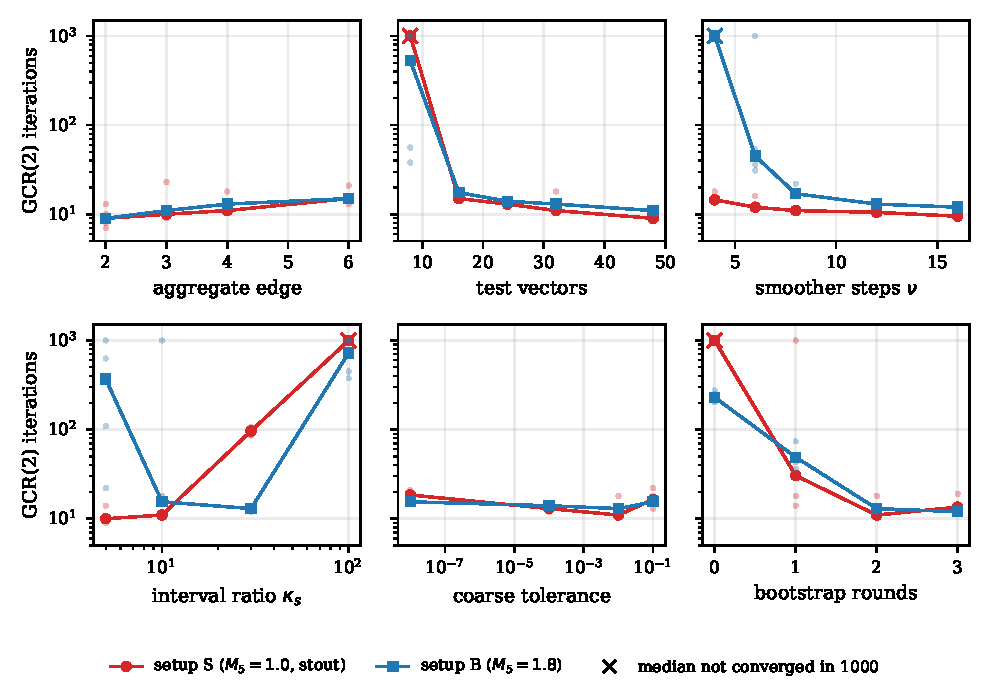
\includegraphics[width=\linewidth]{fig_sensitivity}
\caption{GCR(2) iterations on $\AL$ when one parameter of Table~\ref{tab:setups} is changed,
$12^4$, $m=0.001$, one random right-hand side. Lines: median over the four configurations; dots: the
four configurations; a cross marks a median that does not converge in $1000$ iterations. The default
is the point where the lines of the two setups pass through $14$ iterations. Values and setup and solve
times in Table~\ref{tab:costs}.}
\label{fig:sensitivity}
\end{figure}



Fewer iterations are not always less time (Table~\ref{tab:costs}). Smaller aggregates and more test
vectors save iterations, but the larger coarse space makes the setup and each iteration longer.
On $24^3\times48$, $16$ test vectors do not suffice: the solve needs hundreds of iterations or does
not converge in $2000$. Outside the window the failures can come from the outer solver alone. With
$\kappa_s=10$ in setup~B, one of the four $12^4$ configurations brings GCR(2) to a plateau; with the
same cycle GCR(16) converges, and other setup seeds converge with GCR(2).

Whyte, Stathopoulos and Romero~\cite{WhyteSVD} obtain, for Wilson fermions, the effect of more test
vectors at the coarse size of fewer by truncating them with a singular value decomposition on each
aggregate. Here the truncated basis would no longer contain $s$ and $\hat t$ exactly; whether the
gain outweighs that loss is open.

\subsection{Why the method converges}
\label{sec:why}

The convergence is set by the spectrum and the pseudospectra of the preconditioned operator, not
by its field of values. On the smeared lattices the field of values of $\AR\mathcal M$ reaches into
the left half-plane, so the bound of Eisenstat, Elman and Schultz~\cite{ESS} for GCR does not apply.
Its eigenvalues lie at $\Re\lambda\ge0.70$ with moderate condition numbers, and its pseudospectra
bound full GMRES. As usual for multigrid preconditioners of lattice Dirac operators, the
convergence of the truncated flexible outer method is established numerically.

Two notions from non-Hermitian linear algebra are used. The \emph{field of values}
$W(X)=\{z\dg Xz/z\dg z\}$ contains the spectrum, and its leftmost point is the smallest eigenvalue
of the Hermitian part $(X+X\dg)/2$; GCR converges at every restart length when $W$ lies in the
right half-plane~\cite{ESS}. The \emph{$\varepsilon$-pseudospectrum} is the set of $z$ where
$\sigma_{\min}(z-X)<\varepsilon$; for a normal $X$ it is the $\varepsilon$-neighborhood of the
spectrum, for a non-normal one it can be much larger, and it bounds full
GMRES~\cite{TrefethenEmbree}. The condition number of an eigenvalue, $\kappa=1/|y\dg x|$ for its
normalized right and left eigenvectors, is $1$ for a normal matrix and widens the pseudospectrum
around the eigenvalue.

The quantities of this subsection take $\mathcal M$ as a fixed linear map: both coarse factors solved
to $|r|^2/|b|^2<10^{-20}$ in double precision, the Pauli--Villars factor regularized as in
Eq.~\eqref{eq:tikhonov}, and $\mathcal M\dg$ built as its adjoint, so that
$\langle z|\AR\mathcal M w\rangle$ and $\langle\mathcal M\dg\AR\dg z|w\rangle$ agree to $10^{-10}$.

\subsubsection{Field of values: the coarse correction amplifies}
\label{sec:fov}

The coarse correction pushes the field of values into the left half-plane (Table~\ref{tab:fov}).
The field of values of $\AR$ itself reaches only just below zero and hardly depends on the volume,
and the smoother is harmless, $\|I-\AR\mathcal S\|\approx1$. The coarse correction $E$ is the identity
on the vectors it is built from (Eq.~\eqref{eq:exact}) but amplifies other directions, like a
strongly oblique projection, by three orders of magnitude. The post-smoothing acts as a filter
and brings the whole cycle back close to the identity. Eick and Mawhinney~\cite{EickMawhinney}
describe the same mechanism for a renormalization-group coarse lattice and need a Chebyshev filter
of high degree; here $\AR$ is close to the identity on the high modes, and the smoother suffices.

With stout smearing $W(\AR\mathcal M)$ crosses the origin on every configuration. Without smearing
the amplification is far smaller and $W(\AR\mathcal M)$ lies in the right half-plane, where
truncated GCR($k$) is guaranteed to converge for every $k$~\cite{ESS}.

\subsubsection{Spectrum: far from the origin}
\label{sec:spectrum}

The spectrum, unlike the field of values, stays far from the origin (Table~\ref{tab:spectrum},
Fig.~\ref{fig:spectrum}). Every eigenvalue lies at $\Re\lambda\ge0.70$, with moderate condition
numbers. Setup~S has one or two isolated outliers of larger modulus, and all other eigenvalues lie in
a disc about $1$ that excludes the origin. The left and right forms have nearly the same spectrum.

\subsubsection{Pseudospectra and a bound for GMRES}
\label{sec:pseudo}

For a non-normal operator the eigenvalues alone do not bound the convergence of
GMRES; the $\varepsilon$-pseudospectrum, the set where $\sigma_{\min}(z-X)<\varepsilon$,
does~\cite{NRT,TrefethenEmbree}. If a contour $\Gamma$ of length $L$ encloses the
spectrum of $X$ but not the origin and $\sigma_{\min}(z-X)\ge\varepsilon$ on it, then
for any polynomial $p_k$ with $p_k(0)=1$,
\begin{equation}
\frac{\|r_k\|}{\|r_0\|}\le\|p_k(X)\|\le\frac{L}{2\pi\varepsilon}\max_{z\in\Gamma}|p_k(z)| .
\label{eq:pseudobound}
\end{equation}
An isolated outlier $\lambda_o$ outside $\Gamma$ is removed by the factor
$(1-z/\lambda_o)$ of $p_k$: then $p_k(X)=p_k(X)(I-P_o)$ with $P_o$ the spectral
projector, $\|(z-X)^{-1}(I-P_o)\|\le\kappa_o/\varepsilon$, and with a circle
$|z-c|=r$ and $p_k(z)=(1-z/\lambda_o)(1-z/c)^{k-1}$,
\begin{equation}
\frac{\|r_k\|}{\|r_0\|}\le\kappa_o\,\frac{r}{\varepsilon}\,
\frac{|\lambda_o-c|+r}{|\lambda_o|}\Big(\frac rc\Big)^{k-1}.
\label{eq:outlierbound}
\end{equation}

\begin{figure}[t]
\centering
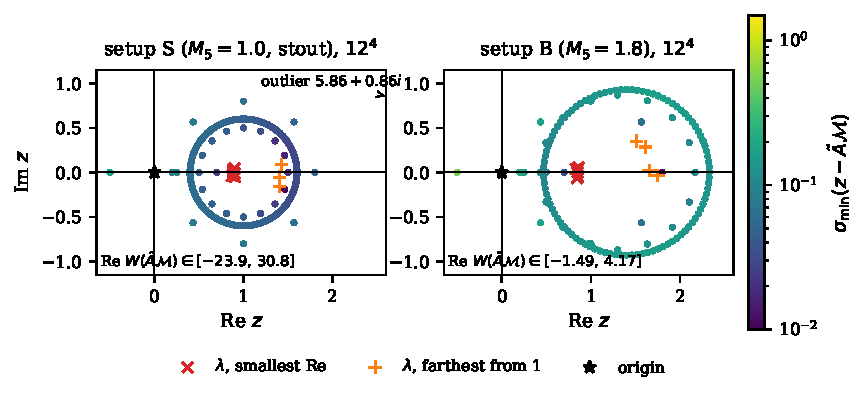
\includegraphics[width=\linewidth]{fig_spectrum}
\caption{$12^4$, $m=0.001$, exact coarse solves (the Pauli--Villars factor regularized): the six eigenvalues of
$\AR\mathcal M$ of smallest real part, the four farthest from $1$, and
$\sigma_{\min}(z-\AR\mathcal M)$ (color) at the points where it was computed: the contours of
Table~\ref{tab:pseudo}, among them the dense circles $|z-1|=0.6$ (S) and
$|z-1.4|=0.93$ (B). The field of values reaches far into the left half-plane (its real
range in the corner), the spectrum does not.}
\label{fig:spectrum}
\end{figure}

On $16^4$ setup~S has two outliers; the factor $\kappa_o$ is then replaced by
$\|I-P_1-P_2\|\le1+\kappa_1+\kappa_2$ and there are two factors of the form
$(|\lambda_o-c|+r)/|\lambda_o|$. On the dense circles of $12^4$ the spacing of the points is small
enough that, $\sigma_{\min}(z-X)$ being $1$-Lipschitz in $z$, the bound holds on the whole circle; it
guarantees $\|r_k\|/\|r_0\|<10^{-9}$ within $55$ (S) and $57$ (B) iterations (Table~\ref{tab:pseudo}).

The bound guarantees convergence at a fixed rate, $r/c$ per iteration, with no stagnation. Its rate,
$r/c=0.5$--$0.6$ in setup~S, is close to the one we measure on $24^3\times48$ on configurations 1 and
3, where the median factor per GCR step of $|r|^2$ is $0.23$--$0.41$ (Fig.~\ref{fig:history}), that
is $0.48$--$0.64$ in $|r|$; configuration~2 in setup~S converges more slowly. The Lanczos estimates approach $\sigma_{\min}^2$ from above, the disc rests on the
eigenvalues farthest from $c$ found by Arnoldi, and the bound is for full GMRES with a fixed
$\mathcal M$.

\subsubsection{Truncated GCR and inexact coarse solves}
\label{sec:gcrk}

Truncated GCR does not need accurate coarse solves. With the usual coarse solves to $10^{-2}$,
GCR(2) needs at most one iteration more than GCR(32) on $12^4$ (Table~\ref{tab:gcrk}). Coarse solves
to $10^{-8}$, where $\mathcal M$ is close to the fixed map, do not help: GCR(2) then needs $19$
iterations and GCR($\ge16$) $15$.

Where $E$ amplifies, the solver's cycle is better than the fixed map. At the vector $x$ at the left
end of $W(\AR\mathcal M)$, coarse solves to $10^{-2}$ reduce $\|(I-\AR E)x\|$ by large factors against
exact ones and in most cases make $\Re\,x\dg\AR\mathcal Mx$ positive. With Krylov coarse solves stopped
early the cycle is not a fixed linear map, so this holds for these vectors only.

A truncated method has no guarantee when the field of values contains the origin~\cite{ESS,Embree}.
With a fixed cycle GCR(2) can reach a fixed point, where the new direction is orthogonal to the
residual and the next step repeats it. With the parameters of Table~\ref{tab:setups} no run reached
a plateau. The one plateau we checked, at $\kappa_s=10$ in setup~B (Sec.~\ref{sec:sensitivity}), is
of this kind: the same cycle converges with GCR(16).

\paragraph{Setup seeds.} With the regularized Pauli--Villars solve no setup is slow on $12^4$
(Sec.~\ref{sec:pvcoarse}). Configuration~2 of $24^3\times48$ needs more iterations than the other
three (Table~\ref{tab:volume}); which property of that configuration causes this is open.

\begin{figure}[t]
\centering
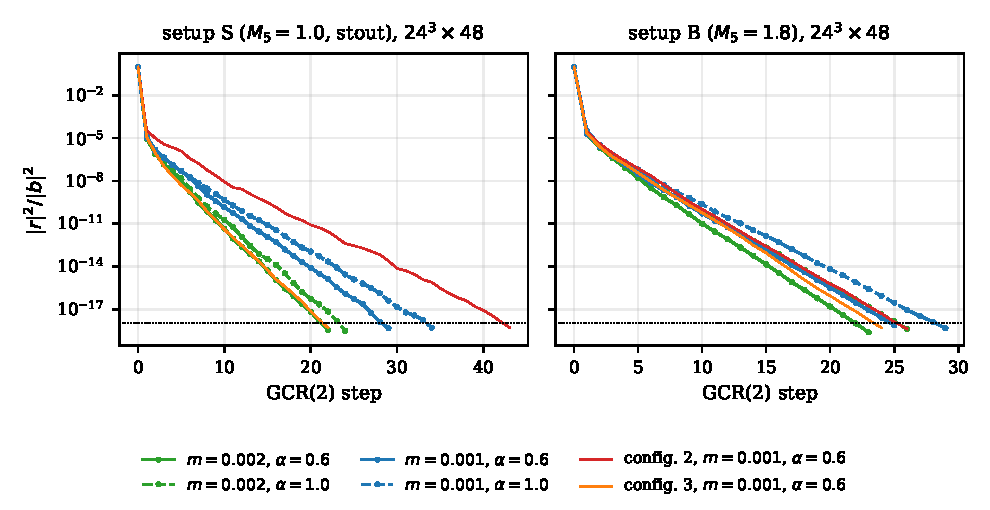
\includegraphics[width=\linewidth]{fig_history}
\caption{GCR(2) residual histories on $24^3\times48$, $\AL$, the multigrid of Table~\ref{tab:setups}: configuration~1 (blue, green) and configurations 2 and 3 at $m=0.001$, $\alpha=0.6$ (red, orange).}
\label{fig:history}
\end{figure}

On $24^3\times48$ no run shows a plateau (Fig.~\ref{fig:history}).
